
\chapter{The Corina server}
\label{txt:servermaintenance}

For basic day-to-day running of the Corina server, you simply need to make sure that the server is running.  All other interaction and managment (creating users, granting permissions, accessing data) is done through the Corina desktop application.  This section, however, outlines a number of aspects of the server that advanced users may find useful.

\section{Backing up and restoring your database}
\index{Server!Backup}
\index{Backup}
As with any computer system it is important for you to back regular backups of your data to guard against hardware (as well as human!) errors. The two main methods for doing this are outlined below:

\subsection{Backup whole Virtual Appliance}
\label{txt:BackupVA}
The simplest method is to make a copy of your entire Virtual Appliance, but this does have a number of drawbacks.  The first is that you need to shut down your server before you can make the backup so this is only possible if server `downtime' is not a problem for your lab.  The second drawback is that it makes a copy of your entire server including the whole operating system, therefore each backup takes a lot more space.  

\begin{enumerate*}
 \item Open VirtualBox
 \item If you server is running you will need to do a full shutdown.  From the server console type \verb|sudo shutdown now| or alternatively you can close the console window and select `Power off the machine'.  This second method is not recommended though as it is like pulling the power plug from the virtual computer.
 \item Select your virtual machine in the list on the left and go to \menutwo{File}{Export Appliance}.
 \item Follow the wizard, specifying a file where you'd like to back the server up to.  Keep in mind that this will contain a complete copy of the server (including operating system) so could be 1Gb or more.
\end{enumerate*}

\subsection{Restoring a Virtual Appliance backup}
If you have followed the instructions in section \ref{txt:BackupVA} to backup your Virtual Appliance the steps to restoring your server are very similar to how your initially installed it.  Simply open VirtualBox, then go to \menutwo{File}{Import Appliance} and select the backup file that you made.  Follow the wizard and it should restore your server.  You can restore onto the same computer that was originally running the virtual machine (remember to give it a new name though if this is the case) or alternatively to any other computer with VirtualBox installed.  This method can therefore be used to share entire databases.


\subsection{Backup PostgreSQL database}
The more standard way of backing up your database is to do a dump of the PostgreSQL database itself.  This is a little more involved, so it is only recommended if you are familiar with command line and/or Linux.

\subsection{Restoring a PostgreSQL database}

\section{Extending the Virtual Appliance}
\index{Server!Graphical interface}
For those of you that are unfamiliar with Linux, the basic command line prompt is not likely to be very comfortable.  If you are interesting in looking at the server in more detail you may therefore prefer to install a full graphical interface.  Unlike Windows, there are a number of different graphical interfaces (or desktops) to choose from in Linux, the most popular being Gnome and KDE.  To install one of these you need to type one of the commands listed below.  The first line installs Gnome and the second KDE. Windows users that are new to Linux may find KDE more familiar, but Apple users may be more at home with Gnome.

 \code{sudo apt-get install ubuntu-desktop}
 \code{sudo apt-get install kubuntu-desktop}

\section{Security}
\index{Security}
The basic installation of the Corina server includes the standard configuration for Apache, PHP and PostgreSQL.  Although these products are considered secure by default, there are a number of measures that can be taken to make them more so.  If your server is only accessible within your local intranet (e.g. behind a robust firewall) then you may not feel it necessary to modify the standard setup.  Precautions may be deemed more important if you server is accessible from the internet.  In this case it would be wise to contact your local network administrator for further information.

\subsection{Usernames and passwords}
\label{txt:passwords}
\index{Passwords}
There are a number of default usernames and passwords setup on your server.  If your server is accessible for the internet we strongly advise you to change these defaults and anyone with knowledge of the Corina server could access and compromise your machine.

\begin{description*}
 \item[System user] - these are the credentials you use to log in to the command prompt in your Corina Virtual Appliance.  By default the user is `corina' and the password is `w3l0v3tr33s'.  To change this log in to the command prompt and type \verb|passwd| and follow the instructions.  There is no way to recover this password if you loose it.
 \item[PostgreSQL database user] - these are the credentials used by the webservice to read and write to the database and are set by the database administrator during the initial configuration of the Corina server. They are also the credentials you will need if you want to directly access the database from a third party tool like PGAdminIII.  You can To reset this password 
 \item[Corina admin user] - these are the admin credentials that you use to log in with in your Corina desktop application.  Be default the user is `admin' and the password is `qu3rcu5'.  To change these open the Corina desktop application, then go to Admin then Change password.
\end{description*}

\subsection{Authentication and encryption}
\index{Authentication}\index{Encryption}
Corina uses a relatively sophisticated method to ensure that unauthorised users cannot access the Corina database through the webservice.  It is loosely based around http digest authentication and uses a challenge and response scheme.  This makes use of cryptographic hashes (a relatively short digital fingerprint of some data but which cannot be decompiled to retrieve the original data) and nonces (a pseudo-random string used just once). All hashes used in the Corina webservice use the MD5 algorithm. This decision will be periodically reviewed to ensure that MD5 is the most appropriate and secure algorithm to use. Whilst an MD5 hash of a short phrase can be compromised, the length and randomness of the original data means with current cracking techniques this is essentially impossible.   For a complete description of Corina's authentication procedure see section \ref{txt:authentication}.

The default Corina server setup, however, uses standard HTTP protocol to communicate between the server and the desktop application.  This is the same protocol used for the majority of web pages on the internet and a determined hacker could eavesdrop on this communication.  Depending on how important and private you perceive your data you may choose to use Secure Socket Layer (SSL) to encrypt this communication.  This is the same technology used by websites such as online banking.  To make full use of this upgrade in security you will however also require a SSL certificate from an official licensing authority.  These certificates typically cost several hundred dollars per year. 


% TODO Describe how to enable SSL

\section{Directly accessing the database}
\index{Database}
\index{PostgreSQL}
Although the Corina database is designed to only be accessed by the Corina desktop application via the Corina server's webservice, you may decide that you'd like to directly access the database yourself.  For instance, you may like to write complicated SQL queries to probe your database in ways not currently supported by the Corina desktop client. 

\warn{Any changes made to the database may have drastic consequences.  We strongly recommend that you never write changes directly to the database as this can cause loss of data and corrupt future upgrades to Corina.}

\subsection{PGAdminIII}
\index{PGAdminIII}
One of the easiest ways to access the PostgreSQL database is through the application PGAdminIII.  This is a cross-platform open source application for communicating with PostgreSQL databases.  You can install PGAdminIII on your desktop computer and access the remotely running database using your database user credentials.  

For security reasons by default the Corina database cannot be accessed from computers outside of the Corina server.  The may sound peculiar because the webservice can be accessed from computers anywhere on the web, but the database is actually accessed by the webservice, which is essentially a user running on the same computer as the database.  To access the database \emph{directly} from a remote computer you must therefore open access first.  This is done by adding an entry to the file `/etc/postgresql/8.4/main/pg\_hba.conf'.  My personal command line text editor of choice is vim, but it is a little confusing to the uninitiated.  If you are unfamiliar with command line text editing you are probably best to use pico:

\code{sudo pico /etc/postgresql/8.4/main/pg\_hba.conf}

Scroll down passed all the comments, to the bottom of the file.  Add the following line:

%%TODO Check this is the best to suggest
\code{host  all  all   IPADDRESS/32       md5}

Make sure you replace IPADDRESS with the IP address of the computer you are trying to connect \emph{from}. This is just one style of pg\_hba.conf entry.  There are many others which allow you to restrict to specific users, computers, networks etc.  See the online PostgreSQL documentation for more details.  Save your changes and exit by doing CTRL+X, then restart the Corina server:

\code{sudo corina-server --restart}

You should now be able to access your database through PGAdminIII. To do this open the application and go to \menutwo{File}{Add server}.  Specify your server's IP address is the host field, and your database username and password.


\subsection{ODBC}
\index{ODBC}
It is also possible to connect to your Corina database via an ODBC connection.  This allows limited access to the database from a variety of database applications including programs like Microsoft Access for which further details are given here.   To use ODBC you will need to install the PostgreSQL ODBC driver (\url{http://www.postgresql.org/ftp/odbc/}) on your desktop computer.

Once you've installed the driver you can then open a blank database in Access and go to Files, Get external data then Link tables.  In the file dialog box change the file type to ODBC Databases().  Next, select the PostgreSQL Unicode driver, then fill out the server details.  You should then be able to open the tables and views from the Corina server database directly from within Access as if they were local tables.  Be warned though that Access and ODBC have many limitations compared to PostgreSQL, especially with regards data types.  For this reason we \emph{strongly} recommend using this for read only purposes.  Using the ODBC connection to write changes to your PostgreSQL database is quite likely to cause serious issues. 

\subsection{PSQL}
\index{PSQL}
The final, and most advanced method is to use the psql client on your server.  This is a command line client which can be used to interrogate the database.  If you're not already familiar with psql it is unlikely that this is a good method for you to use!


\section{Corina server configuration}
\label{txt:serverConfig}
\subsection{Standard server configuration}
\index{config.php}
The Corina server can be configured using the command line tool that is installed on both the Virtual Appliance and native server installs.  It is the same tool that is run at the end of the native server install, but can be run at any time to reconfigure or test your system.  It must be run with superuser privileges therefore \verb|sudo| is required before the command.  For instance to get help on usage type:

\code{sudo corina-server --help}

\begin{wrapfigure}{r}{0.5\textwidth}
  \begin{center}
    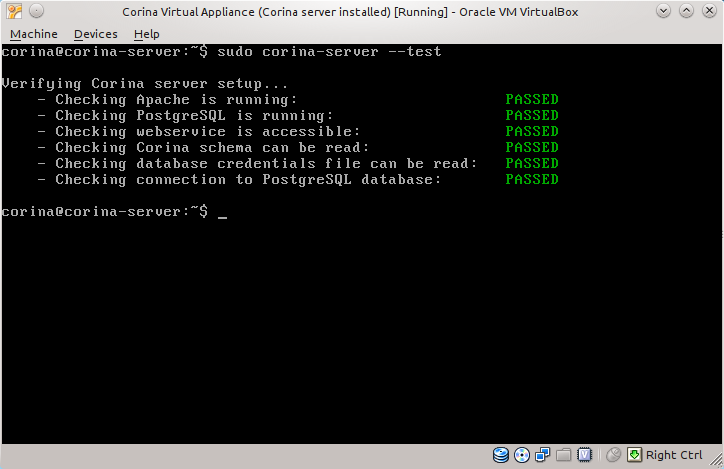
\includegraphics[width=0.48\textwidth]{Images/corina-server-terminal.png}
  \end{center}
  \caption{Example of the output from the corina-server test.}
  \label{fig:serverTerminal}
\end{wrapfigure}

Possible options to pass the server are:

\begin{itemize*}
 \item `\verb|--help|' -- Display a list of the possible options
 \item \verb|`--test'| -- Run tests on the current configuration
 \item \verb|`--configure'| -- Configure the Corina server from scratch.  
 \item \verb|`--reconfigure'| -- Reconfigure the Corina server.  This should be done if the database name or user credentials change, or if the IP address of the machine is altered.
 \item \verb|`--start'| -- Start the Corina server
 \item \verb|`--stop'| -- Stop the Corina server
 \item \verb|`--restart'| -- Restart the Corina server
\end{itemize*} 

Figure \ref{fig:serverTerminal} shows an example of asking the server to test the configuration, with all tests passed successfully.

The command line tool stores the majority of settings in the config.php file stored in the base directory of your Corina webservice.  In theory you could make changes direct to this file, but we do not recommend this unless you know exactly what you're doing.


\subsection{Advanced server configuration}
\index{systemconfig.php}

In addition to the standard configuration options offered on the command line there are a number of other options that can be set.  These are not accessible via the command line because as a rule they should only be altered the Corina developers.  They are primarily for use by the developers as an alternative to hard coding values within the server files.  For instance, one such value is the TRiDaS version being used by the server.  This value will only ever need to be changed alongside other substantial changes to the code.  




\section{Managing map services}
\label{txt:managingmaps}
\index{Web Map Service (WMS)}
\index{Mapping!Adding layers|see{Web Map Service(WMS)}}

There is currently no interface in Corina that lets you specify the WMS mapping services that should automatically be available to your Corina users.  Each user can add servers temporarily (see section \ref{txt:userAddWMS}) but these will disappear at the end of each session.  
